\chapter{Evaluation}

\section{Evaluation Design}


\subsection{Mixing Time Evaluation}
  \begin{itemize}
    \item List the types Traceplot, Densityplots, Gelbin and Rubin multiple sequence diagnostics
    \item Performed Geweke Diagnostic
  \end{itemize}
\subsection{Reconstructions As a measure of Performance}

 \begin{itemize}
   \item Cite literature where reconstructions are used, starting from early RBM training papers by Hinton, up to more recent in deeper networks - the goal being to show the reader that reconstructions are used well in practice.
 \end{itemize}

 \subsection{Growing Complexity of tasks}

 \begin{itemize}
   \item Same models
   \item Growing dimensionality, bit strings to 2d to MNIST
   \item Allows comparison of Approx corrections in smaller scale - fail there don't continue using them...
 \end{itemize}

\section{Evaluation Methods}

My \todowording{x experiements} all followed the same high level process, working from trivial cases to more challenging tasks. The reasoning being that trivial cases make unit testing feasible, therefore ensuring conclusions can be drawn with regard to the algorithm and model, not an incorrect implementation.

The following evaluations aimed to evaluate the ORBM and it's inference algorithm by examining reconstructions given a multi-cause input. An example of a muli-cause input with two quadrilaterals is shown in figure \ref{F:Composite-Example}. The optimal reconstructions are equivalent to the two images that combined form the input.

\begin{wrapfigure}{r}{0.6\textwidth}
  \begin{center}
    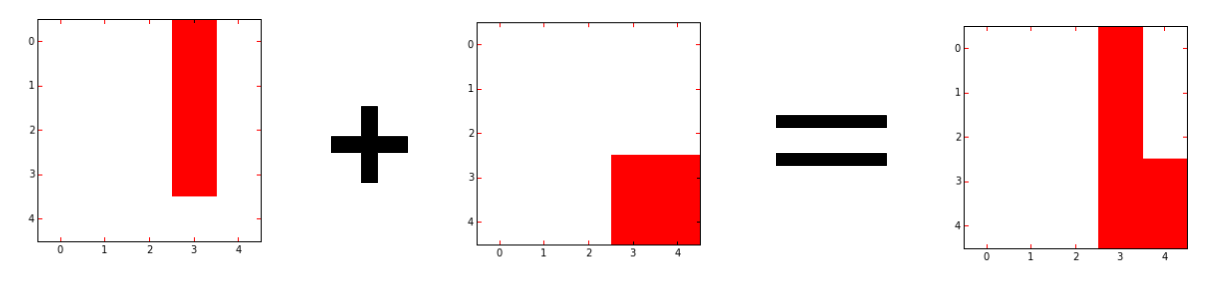
\includegraphics[width=0.48\textwidth]{Assets/Composite-Example.png}
  \end{center}
  \caption{A figure illustrating two five by five pixel images combining to form a composite/multicause input. The images are binary.}
  \label{F:Composite-Example}
\end{wrapfigure}

In the smaller dimenisonal cases the reconstructions are inspected by hand, manually plotting the reconstructions and the frequency with which they occurred after a large amount of repetitions. In the larger dimensional tasks, two `scores` were used to evaluate reconstructions against the training set.

To be able to use this reconstruction based evaluation, knowledge of the ground truth was required. This was so:
\begin{itemize}
  \item RBMs could be trained and then plugged into the ORBM network.
  \item Reconstructions could be compared directly (by score) to the ground truth.
\end{itemize}

\section{Starting from the minimal case, two bit XOR }

\subsubsection{Description}

The starting point for the evalatuion was examining the ORBM reconstructions in a two bit pattern, where two of the same model were combining to form the data. This model made one bit on in a two bit pattern at a time. That is it could either make $[1 , 0]$ or $[0 , 1]$. The training set is the two bit XOR truth table.



\begin{figure}{h}
  \begin{center}
    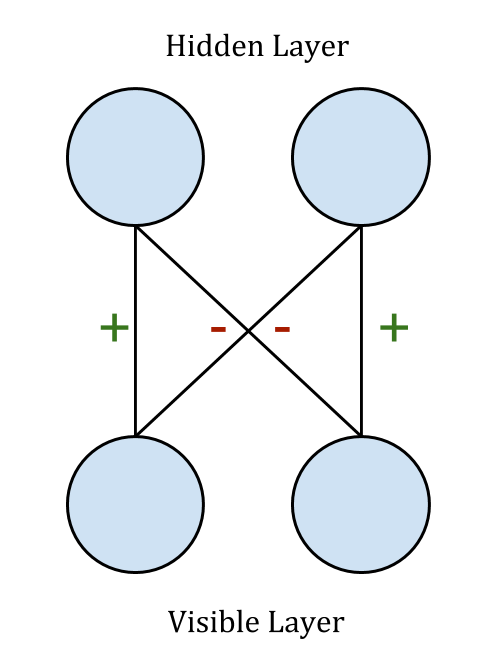
\includegraphics[width=0.3\textwidth]{Assets/Two-Bit-RBM.png}
  \end{center}
  \caption{The two bit RBM for modelling a single bit on at a time in a two bit pattern. The diagonal weights are negative and the non-diagonal weights are positive.}
  \label{F:Two-Bit-RBM}
\end{figure}

\subsubsection{Architecture and Parameters}

\begin{wrapfigure}{l}{0.6\textwidth}
  \begin{center}
    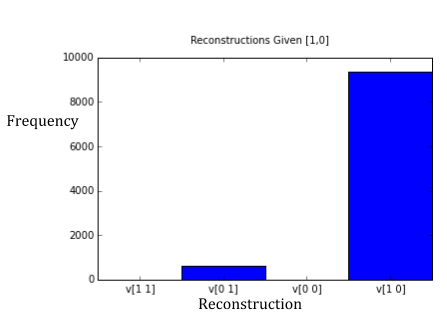
\includegraphics[width=0.5\textwidth]{Assets/Two-Bit-RBM-Recon.png}
  \end{center}
  \caption{Example reconstructions for the Handcrafted RBM, For 10000 independant reconstructions given the input $[1,0]$.}
  \label{F:Two-Bit-RBM-Recons}
\end{wrapfigure}

Being a trivial dimensionality, the RBMs weights were constructed by hand, meaning that only the ORBMs inference algorithm was being evaluated and not the training of the RBMs plugged into it. This network is picture in figure \ref{F:Two-Bit-RBM}, \todowording{with weights greater than 5} the networks stable state results in either $[1 , 0]$ or $[0 , 1]$. The RBMs had 2 hidden units and 2 visible units.

\subsubsection{Method}

This RBM was checked to ensure that it behaved in practice by ensuring it's reconstructions matched the input for a large frequency of reconstructions. The results of trying this with the input $[1,0]$ are showing in figure \ref{F:Two-Bit-RBM-Recons}. The most common reconstruction is  $[1,0]$, which matches the input. We see that $~500$ reconstructions out of the $10,000$ reconstructions were incorrect, corresponding to $[0,1]$. This is due to the stochastic nature of the RBM.



In a similar way to the reconstructions, ancestral samples can be taken from the model and evaluated. \todowording{In larger dimensions Hinton has shown RBMs to be poor generative models without the extra layers above...} however in the small dimensions of this task the dreams should match the training set:

A histogram of frequencies of reconstructions given the RBM is in the free phase, is shown in figure \ref{F:Two-Bit-RBM-Dreams}. Again the model behaves as expected, generating dream patterns that match the training dataset the majority of the time. There is a lack of parity in that the RBM produces the visible pattern $[1,0]$ almost double the time of the visible $[0,1]$, however this is resolved when the generative model is run for longer, and more samples are taken.


\begin{wrapfigure}{r}{0.4\textwidth}
  \begin{center}
    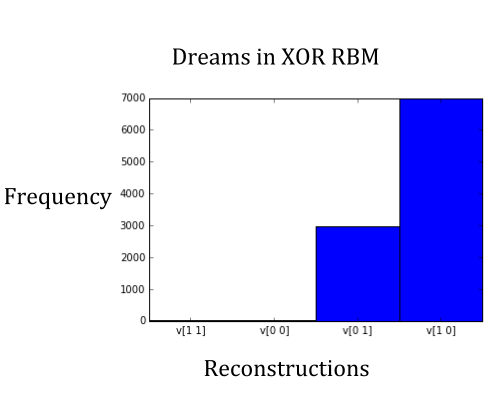
\includegraphics[width=0.35\textwidth]{Assets/XOR-RBM-Dreams.png}
  \end{center}
  \caption{Dreams in the XOR RBM, note how only the training data is present.}
  \label{F:Two-Bit-RBM-Dreams}
\end{wrapfigure}


Given this good model, the XOR RBM was duplicated and plugged into the ORBM structure as picture in figure \ref{F:XOR-ORBM}.


\begin{wrapfigure}{l}{0.55\textwidth}
  \begin{center}
    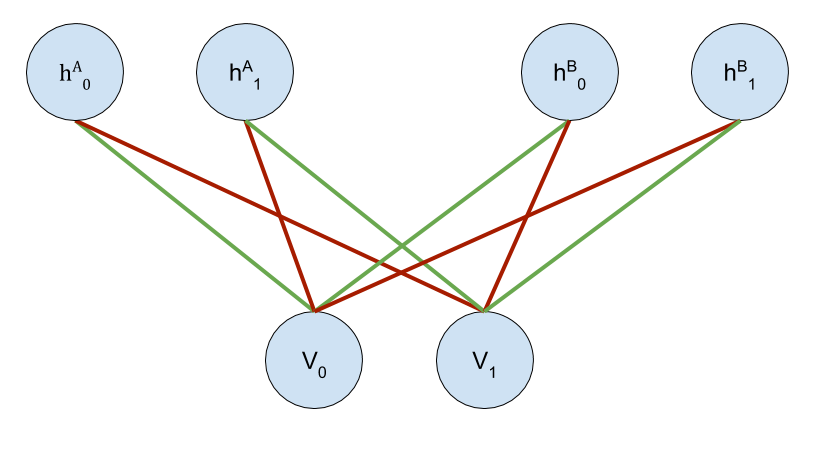
\includegraphics[width=0.5\textwidth]{Assets/XOR-ORBM.png}
  \end{center}
  \caption{Figure showing how the XOR RBM fits into the ORBM architecture.}
  \label{F:XOR-ORBM}
\end{wrapfigure}

The inference algorithm was run in the ORBM architecture for various visible inputs, giving two hidden vectors for the two representations $h^A$ and $h^B$. For each pair of hidden vectors, a reconstruction was created, the process illustrated in figure \ref{F:Two-Bit-ORBM-Inference-REsults-1}. This process was repeated in a similar way to how the reconstructions were evaluated in the lone RBM, counting the frequency each reconstruction occurred over $1500$ runs.

\begin{table}[]
\centering
\begin{tabular}{|l|l|l|}
\hline
Visible Input & \multicolumn{2}{l|}{Expected Reconstructions} \\ \hline
$[1 , 1 ]$    & $[1, 0]$              & $[0,1]$               \\ \hline
$[1, 0 ]$     & $[1,0]$               & $[1, 0]$              \\ \hline
$[0, 1]$      & $[0,1]$               & $[0,1]$               \\ \hline
\end{tabular}
\caption{A Table showing the expected reconstructions from performing ORBM inference with various input patterns. The left and right hand column of the Expected Reconstructions colummn indicate the reconstructions from the left and right RBMs in the ORBM.}
\label{my-label}
\end{table}

\subsubsection{XOR ORBM Analysis}

The results of this process are shown in figure \ref{F:Two-Bit-ORBM-Inference-Results-1}. Where the x-axis shows the reconstructions of the form v\_a$[x,y]$ v\_b$[n,m]$ where $[x,y]$ is the reconstruction (v) created model A and $[n,m]$ is the reconstruction created by model B. The ORBM is able to separate the causes, as the model is being duplicated, it produces $[1,0]$ and $[0,1]$ approximately half the time and symetrically $[0,1]\text{ }[1,0]$ the other half of the time.

\begin{figure}[h]
  \begin{center}
    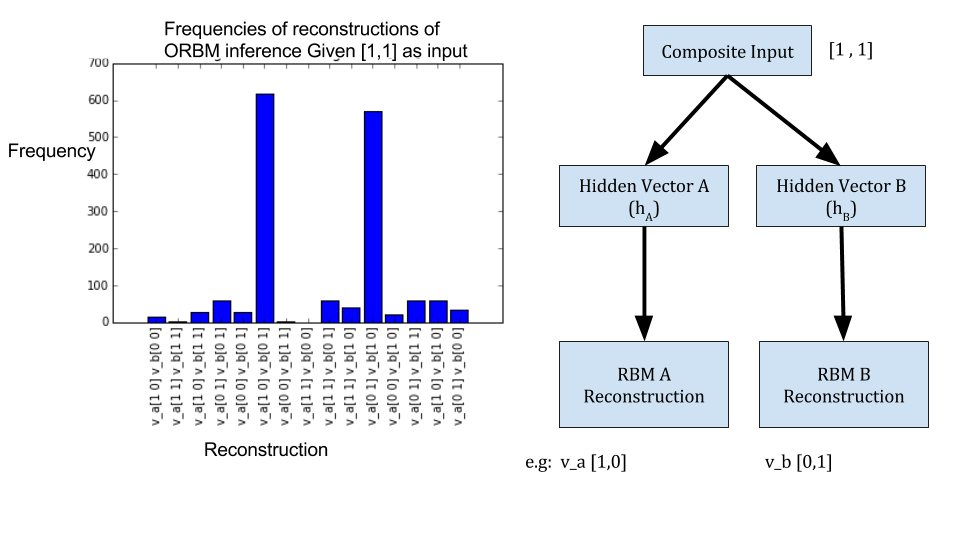
\includegraphics[width=6.5in]{Assets/XOR-2-bit-inference-results.png}
  \end{center}
  \caption{A figure with the results of running ORBM inference 1000 times, showing the frequency for which a given reconstruction occurred. The process is shown in the diagram on the right hand side. }

  \label{F:Two-Bit-ORBM-Inference-Results-1}
\end{figure}

These reconstructions were compared to one of the RBMs trained to recognised a single pattern being on in two bits. As expected a machine that has been trained to recognise one bit, has no concept of two bits being on and hence the reconstructions show no mechanism for seperating the sources. This is illustrated in figure \ref{F:Two-Bit-RBM-Inference-Results-1}.


\begin{figure}[h]
  \begin{center}
    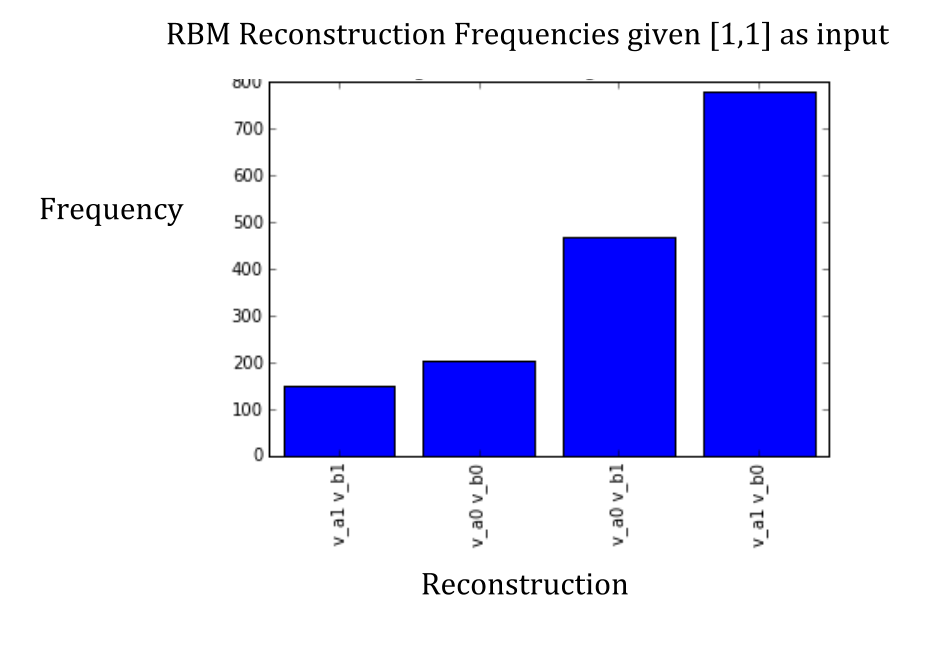
\includegraphics[width=0.8\textwidth]{Assets/RBM-two-bit-XOR-Inference.png}
  \end{center}
  \caption{A figure showing the result of generating 1000 reconstructions with an RBM. It is clear the RBM has no mechanism to separate the sources. Hence showing it [1,1] when it has only been trained on XOR results in no separation, i.e. reconstructions including $[1,1]$.}

  \label{F:Two-Bit-RBM-Inference-Results-1}
\end{figure}

The results of repeating this process with the input $[1,0]$ yielded successful results. We would hope that ORBM architecture could also handle inference with just a single subject. The results of this are shown in
figure \ref{F:Two-Bit-RBM-Inference-Results-2}.\todowording{Do the markers care that it works in this case... it's so trivial does it even mean anything for larger images.}.

\subsubsection{Two bit XOR Conclusion}

The ORBM was able to extract the target patterns $[1,0]$ and $[0,1]$ given the input $[1,1]$. Being the minimal case for source separation, bits in a two bit string, this was important to establish as it meant the approximated correction could be tested and compared. \todowording{Fuck I need to get those pictures in here!}

\begin{figure}[h]
  \begin{center}
    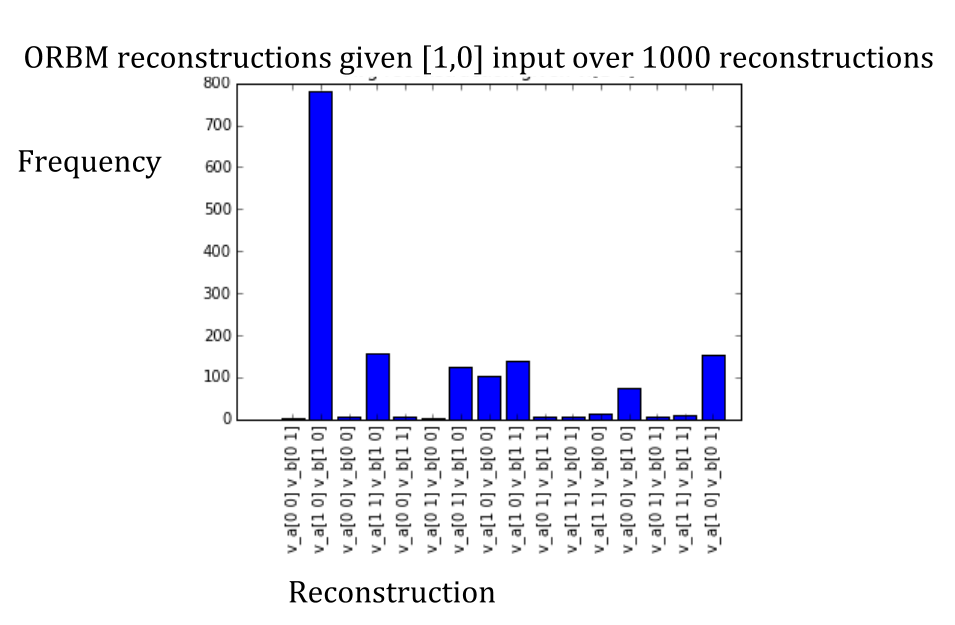
\includegraphics[width=0.8\textwidth]{Assets/ORBM-Reconstructions-[1,1].png}
  \end{center}
  \caption{A figure showing the result of generating 1000 reconstructions with the ORBM with $[1,0]$ as input.}

  \label{F:Two-Bit-RBM-Inference-Results-2}
\end{figure}

\section{$Y$ bit pattern, $X$ neighbouring bits on}

\subsubsection{Description}
A natural next step from a single bit on in a 2 bit pattern, is moving up to $X$  bits side by side on in a $Y$ bit pattern is a next step. For example if $Y = 4 $ and $ X = 2 $ then a valid inputs are the rows of the following:
$$ dataset =
\begin{bmatrix}
  1 & 1 & 0 & 0 \\
  0 & 1 & 1 & 0 \\
  0 & 0 & 1 & 1
\end{bmatrix}
$$

\subsubsection{Architecture and Parameters}
\begin{itemize}
  \item $|Y|$ Hidden units per RBM, any less and we were unable to train the RBM to make the target reconstructions or dreams.
  \item Random normally distributed, mean and standard deviation of one starting weights. The RBM was trained with $1000$ epochs and a learning rate of $0.002$.
  \item A sample of 10,000 dreams were sampled from the RBMs, and then plotted on a histogram in a similar fashion to figure \ref{efnsefskj}. The frequency of these dreams should be roughly equal and the dreams should directly match the training set. This is feasible as the ground truth patterns are known.
\end{itemize}


\subsubsection{Method}

For values of $Y$ where $y \epsilon Y \big| 2 < y < 7$ and all values of $X$ where $x \epsilon X \big| 2 < x < y < 7 $ The process below is repeated.

The inference algorithm was run for 1000 reconstructions in the ORBM architecture for all unique compositions of the training set. The result was 1000 reconstructions per composition of the dataset above. \todowording{Need a way to describe the dataset a bit better}.

\todocite{Need to grab the images out of the ipython notebook.}


\section{2D Patterns in a small dimensional space}
\begin{itemize}
    \item Dataset:
    \begin{itemize}
      \item 2x2 square in a 5x5 image. Dataset of every possible configuration of said square.
    \end{itemize}
    \item Method:
    \begin{itemize}
      \item train a single RBM to represent 2x2 squares in 5x5 space. Nice and small, can still inspect reconstructions, and dreams.
      \item Compose two square images with each other, can the ORBM architecture separate the images.
    \end{itemize}
  \end{itemize}

    \section{2D Pattern, Different Rectangle Separation}
    \begin{itemize}
      \item Dataset
      \begin{itemize}
        \item n by m rectangles in 5x5 Images (TODO-IMAGE-IN-HERE) where n and m are not always equal.
      \end{itemize}
      \item Method
      \begin{itemize}
        \item Superimpose two images as the same way as before. How well can they separate.
      \end{itemize}
    \end{itemize}

    \section{MNIST Digits}
    \begin{itemize}
      \item Dataset
      \begin{itemize}
        \item 500, 28 by 28 pixel, 0-1 valued, handwritten digit images form the training set.
      \end{itemize}
      \item Method
      \begin{itemize}
        \item Train an single RBM per digit (0-9) in the dataset. Each RBM having 100 hidden units, (TODO-CITE-COOKBOOK) for reasoning.
        \item For all 500 training digit images, compose it with every other digit, and itself. This way the ground truth, the sources are known, therefore making evaluation possible.
        \item For all of these compositions us the RBMs trained of the corresponding sources to:
        \begin{itemize}
          \item Compute the RBM reconstructions for the two sources given their composite input. (TODO-SHOW-DIAGRAM)
          \item Compute the ORBM reconstructions, the ORBM using the same RBMs as in the RBM evaluation.
          \item Because 28 by 28 pixels equates to 784 features, emperically examining all reconstructions is non-trivial. Hence some scoring functions are required.
          \item Scoring
          \item Cross Entropy - Approximate the Log likelihood of the underlying dataset.
          \item Pixel Difference Score - Absolute difference in pixels of the image
          \item Cosine Angle - between reconstruction and target vectors. This has the benefit of also being somewhat magnitude agnostic. (TODO-CITE-AS-MEASURE-WITH-JUSTIFICATION).
          \item Repeat this process 30x to give confidence in findings. Scores calculated can then be meaned over the 30 runs.
        \end{itemize}
      \end{itemize}
    \end{itemize}



%   \begin{itemize}
%     \item Method
%     \item Can check the inference algorithm by using RBMs with hand trained weights
%     \item Using a single RBM, copied.
%     \item Diagram with small explaination why RBMs with these weights will work.
%     \begin{itemize}
%       \item 2 Hidden Units, 2 Visible Units. Weights Matrix of [-1,1],[1,-1]
%       \item This ensures that if one visible unit is 1, the other will get set to off.
%     \end{itemize}
%     \item Look at the reconstructions of these RBMs, should match XOR patterns.
%     \begin{itemize}
%       \item 100000 free phase samples from RBMs resulted in [1,0] and [0,1] most of the time. (TODO-SHOW-GRAPHs). 100000 free phase samples is quite quick to calculate for only 4 weights.
%       \item 2 sets of 100000 reconstructions given the patterns [1,0] and [0,1] resulted in all reconstructions for each set producing [1,0] and [0,1].
%     \end{itemize}
%     \item Hypothesis
%     \item Clamp the visible to patterns of interest. Can see the dynamics of the system.
%     \begin{itemize}
%       \item 1,1 This should result in reconstructions matching XOR - [1,0] and [0,1]
%       \item 1,0 This should result in reconstructions of just - [1,0]
%       \item 0,1 Should behave symmertrically to [1,0].
%       \item 0,0 Under the dynamics of the generative model should fall into [0,0].
%     \end{itemize}
%   \end{itemize}
%
%   \subsection{Y Bit pattern, X bits On}
%   \begin{itemize}
%     \item Have to train an RBM to recognise X neighbouring bits on at a time in a Y bit pattern. e.g. X = 2, Y = 5, [0,0,1,1,0]
%     \item num Y hiddens, or more.
%     \item While Y less than 10 it is easy to visualise if separation is occurring.
%   \end{itemize}
%
%   \subsection{2D Pattern, Square Separation, Single Model}
%   \begin{itemize}
%     \item Dataset:
%     \begin{itemize}
%       \item 2x2 square in a 5x5 image. Dataset of every possible configuration of said square.
%     \end{itemize}
%     \item Method:
%     \begin{itemize}
%       \item train a single RBM to represent 2x2 squares in 5x5 space. Nice and small, can still inspect reconstructions, and dreams.
%       \item Compose two square images with each other, can the ORBM architecture separate the images.
%     \end{itemize}
%   \end{itemize}
%
%   \subsection{2D Pattern, Different Rectangle Separation}
%   \begin{itemize}
%     \item Dataset
%     \begin{itemize}
%       \item n by m rectangles in 5x5 Images (TODO-IMAGE-IN-HERE) where n and m are not always equal.
%     \end{itemize}
%     \item Method
%     \begin{itemize}
%       \item Superimpose two images as the same way as before. How well can they separate.
%     \end{itemize}
%   \end{itemize}
%
%   \subsection{MNIST Digits}
%   \begin{itemize}
%     \item Dataset
%     \begin{itemize}
%       \item 500, 28 by 28 pixel, 0-1 valued, handwritten digit images form the training set.
%     \end{itemize}
%     \item Method
%     \begin{itemize}
%       \item Train an single RBM per digit (0-9) in the dataset. Each RBM having 100 hidden units, (TODO-CITE-COOKBOOK) for reasoning.
%       \item For all 500 training digit images, compose it with every other digit, and itself. This way the ground truth, the sources are known, therefore making evaluation possible.
%       \item For all of these compositions us the RBMs trained of the corresponding sources to:
%       \begin{itemize}
%         \item Compute the RBM reconstructions for the two sources given their composite input. (TODO-SHOW-DIAGRAM)
%         \item Compute the ORBM reconstructions, the ORBM using the same RBMs as in the RBM evaluation.
%         \item Because 28 by 28 pixels equates to 784 features, emperically examining all reconstructions is non-trivial. Hence some scoring functions are required.
%         \item Scoring
%         \item Cross Entropy - Approximate the Log likelihood of the underlying dataset.
%         \item Pixel Difference Score - Absolute difference in pixels of the image
%         \item Cosine Angle - between reconstruction and target vectors. This has the benefit of also being somewhat magnitude agnostic. (TODO-CITE-AS-MEASURE-WITH-JUSTIFICATION).
%         \item Repeat this process 30x to give confidence in findings. Scores calculated can then be meaned over the 30 runs.
%       \end{itemize}
%     \end{itemize}
%   \end{itemize}
%
%
% \subsection{Classifciation Accuracy on Hidden Representation}
%   Not sure about this one.
